\input{../style/preamble}
\input{../latex-math/basic-math}
\input{../latex-math/basic-ml}
\input{../latex-math/ml-nn}

% Macros used by earlier sessions' adapted material, kept in sync since this session
% recaps/extends session 7-8 content and reuses the same conventions.
\newcommand{\ques}{\textbf{\textcolor{red}{Question:  }}}
\newcommand{\citebutton}[2]{\beamergotobutton{\href{#2}{#1}}}
\tikzstyle{squ}=[draw, rectangle, minimum size = 5mm]
\tikzstyle{del}=[squ, fill = white]
\tikzstyle{vec}=[draw, rectangle, fill = white, minimum width=5mm, minimum height=1cm, inner sep = 2pt]

\newcommand{\titlefigure}{figure/vit-patches.png}
\newcommand{\learninggoals}{
  \item Vision Transformers: how an image becomes a token sequence, and why CNN's inductive biases (locality, translation equivariance) are a data-efficiency trade-off, not a hard requirement
  \item Making ViT practical: windowed/hierarchical attention (Swin) and training without massive data via distillation (DeiT)
  \item DETR and MaskFormer: object detection and segmentation as set prediction with a non-autoregressive decoder -- a third encoder-decoder pattern alongside T5's and Whisper's autoregressive ones
  \item Two ways to combine modalities: contrastive dual-encoders (CLIP, incl.\ its actual training objective) vs.\ fusion architectures, and where image captioning and text-to-image generation fit
  \item Unified, domain-agnostic architectures (Gato, OFA): the same recipe applied to text, images, robot actions, and arbitrary tasks alike
  \item Video Transformers: factorizing space and time (ViViT, TimeSformer) to keep attention tractable
  \item That every family and pattern from sessions 7-9 generalizes past text -- this was never an NLP-only architecture
}

\title{Advanced Artificial Intelligence and Machine Learning}
\date{}

\begin{document}

\lecturechapter{Transformers Outside NLP}
\lecture{Advanced AI \& ML}
%%%%%%%%%%%%%%%%%%%%%%%%%%%%%%%%%%%%%%%%%%%%%%%%%%%%%%%%%%%%%%%%%%

\section{Recap and Roadmap}
%%%%%%%%%%%%%%%%%%%%%%%%%%%%%%%%%%%%%%%%%%%%%%%%%%%%%%%%%%%%%%%%%%

\begin{vbframe}{Where We Left Off}
\begin{itemize}
  \item Sessions 7-9 covered the Transformer's three families -- encoder-only, decoder-only, encoder-decoder -- entirely through their NLP flagships: BERT, GPT, and T5/the original Transformer.
  \item Session 8 already showed brief evidence this isn't NLP-specific (Vision Transformer, CLIP, Flamingo, GPT-4, Whisper). This session goes deep on \emph{how} those and related non-NLP models actually work.
  \item Running order: Vision Transformers (encoder-only, applied to images) $\to$ DETR (a third encoder-decoder pattern) $\to$ multimodal architectures (combining modalities, two different ways) $\to$ unified architectures (one model, any modality) $\to$ video, briefly $\to$ a final synthesis across all four Transformer sessions.
\end{itemize}
\end{vbframe}

%%%%%%%%%%%%%%%%%%%%%%%%%%%%%%%%%%%%%%%%%%%%%%%%%%%%%%%%%%%%%%%%%%

\section{Vision Transformers, In Depth}
%%%%%%%%%%%%%%%%%%%%%%%%%%%%%%%%%%%%%%%%%%%%%%%%%%%%%%%%%%%%%%%%%%

\begin{vbframe}{From Pixels to Tokens}
\begin{itemize}
  \item ViT's central move (Dosovitskiy et al., 2020): split an image into fixed-size, non-overlapping patches (e.g.\ $16\times16$ pixels), flatten each patch, and linearly project it -- exactly the token-embedding step from session 7, just applied to pixel patches instead of sub-word tokens.
\end{itemize}

\begin{center}
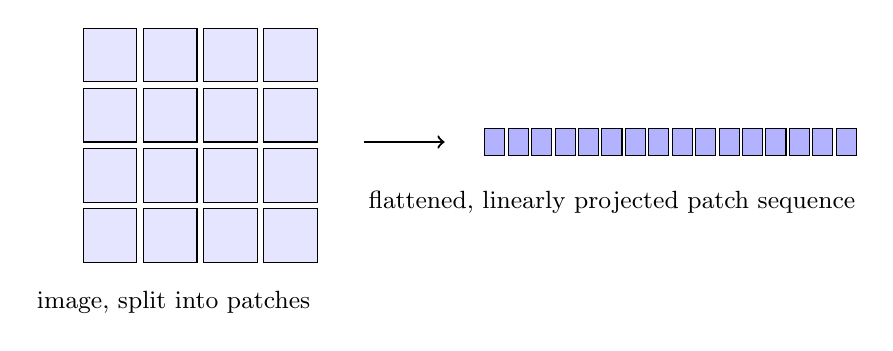
\begin{tikzpicture}[scale=0.85]
  \foreach \x in {0,1,2,3} {
    \foreach \y in {0,1,2,3} {
      \draw[fill=blue!10] (\x*0.9, \y*0.9) rectangle ++(0.8,0.8);
    }
  }
  \node at (1.35, -0.6) {\small image, split into patches};
  \draw[->, thick] (4.2, 1.8) -- (5.4, 1.8);
  \foreach \i in {0,...,15} {
    \draw[fill=blue!30] (6 + 0.35*\i, 1.6) rectangle ++(0.3, 0.4);
  }
  \node at (7.9, 0.9) {\small flattened, linearly projected patch sequence};
\end{tikzpicture}
\end{center}

\begin{itemize}
  \item A learnable {\tt [CLS]} token is prepended (exactly BERT's convention), and a learnable position embedding is added to every patch (position is otherwise lost, per the permutation-equivariance property from session 7 -- 2D images need it just as much as 1D text does).
  \item The result feeds an entirely standard Transformer \textbf{encoder} -- bidirectional self-attention, no architectural changes from session 7 at all. The {\tt [CLS]} token's final representation drives classification, again exactly like BERT.
\end{itemize}

\framebreak

\textbf{Concretely, with real numbers:} a standard $224\times224$-pixel image, split into $16\times16$ patches:
\begin{itemize}
  \item Patches per row/column: $224 / 16 = 14$. Total patches: $14\times14 = 196$.
  \item Plus the {\tt [CLS]} token: a sequence of \textbf{197 tokens} enters the encoder -- about the length of two or three typical sentences in session 7's terms, not the thousands of pixels the raw image has.
  \item Each patch is $16\times16\times3 = 768$ raw numbers (RGB), linearly projected down to whatever embedding size $d_{model}$ the model uses (768 for the original ``ViT-Base'', not a coincidence -- it matches BERT-Base's embedding size exactly).
  \item Intuition for \emph{why} patches at all, instead of one token per pixel: at pixel-level granularity a $224\times224$ image would be a 50{,}176-token sequence, and self-attention's $\mathcal{O}(n^2)$ cost (session 7) makes that hopeless. Patches are the coarsest grouping that still lets the model see the whole image, chosen purely to keep the sequence short enough to attend over.
\end{itemize}
\end{vbframe}

\begin{vbframe}{CNNs vs.\ ViT: Inductive Bias}
\begin{itemize}
  \item \textbf{Inductive bias}: the built-in assumptions a model architecture makes before seeing any data.
  \item CNNs bake in two strong ones: \textbf{locality} (pixels mainly interact with nearby pixels) and \textbf{translational equivariance} (a shifted object still gets recognized the same way, because the same kernel slides over the whole image).
  \item ViT has neither built in -- self-attention connects every patch to every other patch equally from the start, with no notion of ``nearby'' unless the model learns one.
\end{itemize}

\framebreak

\textbf{Making this concrete:} imagine a photo of a cat, once with the cat centered, once with the exact same cat shifted into the bottom-right corner.
\begin{itemize}
  \item A CNN's convolutional kernel is a small filter that slides across the \emph{entire} image using the \emph{same} weights everywhere -- so whatever pattern it learned to detect (an ear, a whisker) is detected wherever it occurs. It never had to see a bottom-right-corner cat during training to recognize one at test time; the sliding-window mechanism gives it that for free.
  \item A ViT patch in the bottom-right corner has its \emph{own} position embedding, entirely separate from the center patches' embeddings. If the model only ever saw centered cats during training, there's no built-in reason a bottom-right cat should be recognized the same way -- the model would have to have \emph{learned}, from examples, that patch content matters more than patch position for this task.
  \item That's the whole trade-off in one picture: a CNN gets ``it doesn't matter where in the image this pattern appears'' for free, by construction. A ViT has to discover that fact from data -- and until it has seen enough varied examples to discover it, it will be worse at exactly this kind of generalization than a CNN is by default.
\end{itemize}

\begin{itemize}
  \item Below a certain dataset size, CNNs win: their inductive biases are simply correct priors for natural images, and ViT has to spend data learning what a CNN gets for free.
  \item Above that threshold, ViT catches up and surpasses CNNs -- self-attention's lack of built-in assumptions becomes an advantage once there's enough data to learn the \emph{right} assumptions instead of a fixed one, and Transformer blocks scale (in compute and in expressiveness) better than convolutions do.
  \item Practical consequence: very few people train a ViT from scratch. The standard workflow is transfer learning from a model already pretrained on a massive dataset -- freeze most weights, fine-tune only the classification head (or, for a bigger domain gap, fine-tune the whole model at a low learning rate).
\end{itemize}
{\footnotesize Framing after Hugging Face's Community Computer Vision Course, \enquote{Vision Transformers for Image Classification} (MIT licensed); Dosovitskiy et al., 2020.}
\end{vbframe}

%%%%%%%%%%%%%%%%%%%%%%%%%%%%%%%%%%%%%%%%%%%%%%%%%%%%%%%%%%%%%%%%%%

\section{Efficient Vision Transformers}
%%%%%%%%%%%%%%%%%%%%%%%%%%%%%%%%%%%%%%%%%%%%%%%%%%%%%%%%%%%%%%%%%%

\begin{vbframe}{Swin Transformer: Windowed Attention}
\begin{itemize}
  \item Plain ViT attends every patch to every other patch -- the same $\mathcal{O}(n^2)$ cost from session 7, now over however many patches a (potentially high-resolution) image needs.
  \item \textbf{Swin Transformer} (Liu et al., 2021) restricts self-attention to small, non-overlapping local windows (e.g.\ $7\times7$ patches): patches only attend within their own window, not globally -- linear complexity in image size instead of quadratic. This is session 7's \textbf{local attention} pattern, used here as the default design, not an optional efficiency add-on.
  \item To still let information cross window boundaries, alternating layers use a \textbf{shifted} window partition -- the windows in layer $l+1$ are offset from layer $l$'s, so patches near a boundary in one layer end up in the same window in the next.
\end{itemize}

\framebreak

\textbf{An intuition for shifting:} imagine reading a book one paragraph at a time, understanding each paragraph fully before moving to the next (that's one layer of fixed windows) -- but an idea that happens to span a paragraph \emph{break} never gets connected, because the two halves are never read together.
\begin{itemize}
  \item Swin's fix: in the very next layer, shift where the ``paragraph breaks'' fall (the window boundaries), so content that was split across two windows before is now inside the same window.
  \item Stack enough of these shifted layers and information has effectively traveled across the whole image, one window-hop at a time -- without ever paying for a single patch to attend to every other patch directly.
  \item This is a cheaper, structured way to reach the same goal Transformer-XL's segment recurrence solved for text (session 7): let information cross a hard boundary the current layer can't see across, without going back to full quadratic attention.
\end{itemize}

\framebreak

\begin{itemize}
  \item \textbf{Hierarchical structure}: between stages, a \texttt{PatchMerging} layer merges groups of neighboring patches and doubles the channel depth -- exactly the resolution-shrinks-while-channels-grow pattern a CNN's pooling layers produce, which plain ViT has no equivalent of (it keeps one fixed resolution throughout).
  \item Consequence: Swin produces a multi-scale feature pyramid, so it plugs directly into detection/segmentation architectures designed around CNN backbones -- one reason it (not plain ViT) became the default Transformer backbone for those tasks. Swin V2 scales to 3B parameters.
\end{itemize}
\end{vbframe}

\begin{vbframe}{Training ViT Without Massive Data: DeiT}
\begin{itemize}
  \item The pain point from two frames ago: ViT needs pretraining on hundreds of millions of images (the original paper used JFT-300M) to beat a CNN. Most labs don't have that.
  \item \textbf{DeiT} (Touvron et al., 2021) trains a competitive ViT on ImageNet-1k alone ($\sim$1.3M images) via \textbf{knowledge distillation} from a CNN teacher.
  \item Mechanism: add a second learnable token -- a \textbf{distillation token} -- alongside the {\tt [CLS]} token. {\tt [CLS]} trains on the true labels as usual; the distillation token trains to match the CNN teacher's prediction. Both attend to the same patch sequence throughout the network.
  \item Same soft/hard-target distillation idea as DistilBERT (session 8) -- but the goal here isn't a smaller model, it's transferring a CNN's locality/translation-equivariance bias into a data-hungry architecture that has none of its own.
\end{itemize}
\end{vbframe}

%%%%%%%%%%%%%%%%%%%%%%%%%%%%%%%%%%%%%%%%%%%%%%%%%%%%%%%%%%%%%%%%%%

\section{DETR: A Third Encoder-Decoder Pattern}
%%%%%%%%%%%%%%%%%%%%%%%%%%%%%%%%%%%%%%%%%%%%%%%%%%%%%%%%%%%%%%%%%%

\begin{vbframe}{Object Detection, the Old Way}
\begin{itemize}
  \item \textbf{Task}: given an image, output a set of (class, bounding box) pairs -- e.g.\ \texttt{[(car, x, y, w, h), (pedestrian, x', y', w', h')]}.
  \item Classical detectors (e.g.\ YOLO): hand-crafted \textbf{anchor boxes} as position/size priors, dense per-cell predictions, then heavy post-processing (non-maximum suppression) to remove duplicate/overlapping boxes.
  \item \textbf{DETR} (Carion et al., 2020) removes all of that: a CNN backbone plus a Transformer encoder-decoder predicts the whole set of boxes directly, in parallel, with (almost) no post-processing.
\end{itemize}
\end{vbframe}

\begin{vbframe}{DETR's Decoder Isn't Autoregressive}
\begin{itemize}
  \item Every encoder-decoder example so far (T5, Whisper) generates its output \emph{autoregressively}, one token at a time. DETR's decoder does not.
\end{itemize}

\begin{center}
\begin{tikzpicture}[node distance=9mm, ->, thick, >=stealth, every node/.style={font=\footnotesize}]
  \node[draw, rectangle, align=center, inner sep=3pt] (cnn) {CNN\\backbone};
  \node[draw, rectangle, align=center, inner sep=3pt, right=of cnn] (enc) {Transformer\\encoder};
  \node[draw, rectangle, align=center, inner sep=3pt, right=of enc] (dec) {Transformer\\decoder};
  \node[draw, rectangle, align=center, inner sep=3pt, right=of dec] (ffn) {per-slot\\FFN heads};
  \node[align=center, below=7mm of dec] (q) {$N$ learned\\object queries};
  \node[align=center, above=7mm of ffn] (out) {class + box\\per slot};
  \draw (cnn) -- (enc);
  \draw (enc) -- (dec);
  \draw (q) -- (dec);
  \draw (dec) -- (ffn);
  \draw[-] (ffn) -- (out);
\end{tikzpicture}
\end{center}

\begin{itemize}
  \item A fixed number $N$ of learned \textbf{object query} vectors (e.g.\ $N=100$) are decoded \emph{simultaneously} via cross-attention over the encoder's output -- one query per potential object, all at once, no left-to-right dependency between them.
  \item Most queries predict a ``no object'' class; the rest predict a real (class, box) pair.
\end{itemize}
\end{vbframe}

\begin{vbframe}{Matching Predictions to Ground Truth: Bipartite Matching}
\begin{itemize}
  \item \ques If predictions come out unordered and in parallel, which predicted box should be compared against which ground-truth box when computing the loss?
  \item DETR finds the one-to-one assignment (a \textbf{bipartite matching}) between the $N$ predictions and the ground-truth objects that minimizes total matching cost (class mismatch + box mismatch), via the Hungarian algorithm -- then computes an ordinary loss on that specific pairing.
  \item Because the assignment is permutation-invariant by construction, DETR never needs anchor boxes or non-maximum suppression: exactly one prediction is trained to match each ground-truth object.
\end{itemize}

\framebreak

\textbf{A small worked example.} Say $N=3$ queries predicted boxes for a photo with 2 real objects (a cat, a dog); one query will be assigned ``no object''.

\begin{center}
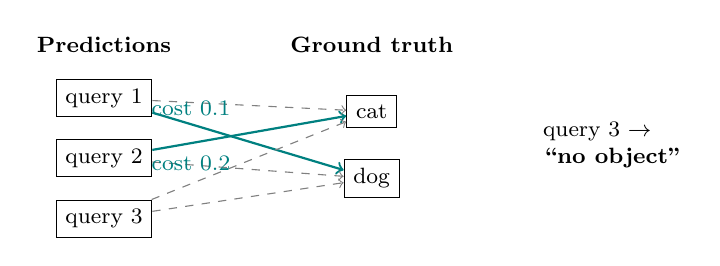
\begin{tikzpicture}[scale=0.85, every node/.style={font=\footnotesize}]
  \node at (0,2) {\textbf{Predictions}};
  \node[draw, rectangle] (p1) at (0,1.2) {query 1};
  \node[draw, rectangle] (p2) at (0,0.3) {query 2};
  \node[draw, rectangle] (p3) at (0,-0.6) {query 3};
  \node at (4,2) {\textbf{Ground truth}};
  \node[draw, rectangle] (g1) at (4,1) {cat};
  \node[draw, rectangle] (g2) at (4,0) {dog};
  \draw[->, thick, teal] (p1) -- (g2);
  \draw[->, thick, teal] (p2) -- (g1);
  \draw[->, dashed, gray] (p1) -- (g1);
  \draw[->, dashed, gray] (p2) -- (g2);
  \draw[->, dashed, gray] (p3) -- (g1);
  \draw[->, dashed, gray] (p3) -- (g2);
  \node[teal] at (1.3,1.05) {cost 0.1};
  \node[teal] at (1.3,0.22) {cost 0.2};
  \node[align=left] at (7.6,0.5) {query 3 $\to$\\\textbf{``no object''}};
\end{tikzpicture}
\end{center}

\begin{itemize}
  \item Every possible pairing (all dashed \emph{and} solid lines) has a cost; the Hungarian algorithm picks the one-to-one assignment (\textcolor{teal}{teal}, solid) with the \emph{lowest total cost} -- here, query 1 $\to$ dog and query 2 $\to$ cat, even though query 1 happened to be listed first and ``cat'' happened to be listed first; the algorithm doesn't care about either ordering, only about the total cost.
  \item Query 3 matches nothing well enough, so it's assigned the ``no object'' class -- exactly the outcome that lets DETR handle images with anywhere from zero to $N$ objects using one fixed-size output.
\end{itemize}
\end{vbframe}

\begin{vbframe}{DETR Is Surprisingly Short Code}
{\footnotesize
\begin{verbatim}
class DETR(nn.Module):
    def __init__(self, num_classes, hidden_dim, nheads,
                 num_encoder_layers, num_decoder_layers):
        super().__init__()
        self.backbone = nn.Sequential(*list(
            resnet50(pretrained=True).children())[:-2])
        self.conv = nn.Conv2d(2048, hidden_dim, 1)
        self.transformer = nn.Transformer(
            hidden_dim, nheads, num_encoder_layers, num_decoder_layers)
        self.linear_class = nn.Linear(hidden_dim, num_classes + 1)
        self.linear_bbox = nn.Linear(hidden_dim, 4)
        self.query_pos = nn.Parameter(torch.rand(100, hidden_dim))
\end{verbatim}}
\begin{itemize}
  \item A ResNet-50 backbone, a single \texttt{1x1} conv to reduce channels, PyTorch's built-in \texttt{nn.Transformer}, and two linear heads -- the ``no anchors, no NMS'' simplicity claim is visible directly in the code, not just in prose.
  \item \texttt{query\_pos}: exactly the $N=100$ learned object queries from the previous frame, as a plain trainable parameter matrix.
\end{itemize}
{\footnotesize Code: Hugging Face Community Computer Vision Course, \enquote{DETR} (MIT licensed), itself adapted from Carion et al., 2020's own minimal implementation.}
\end{vbframe}

\begin{vbframe}{DETR's Evolution}
\begin{itemize}
  \item Original DETR: slow to converge, weaker on small objects.
  \item \textbf{Deformable DETR} (Zhu et al., 2020): each query attends only to a small, learned set of sampling points near a reference point (not every encoder position) -- cheaper, and multi-scale feature maps (as in YOLOv3) fix the small-object weakness.
  \item \textbf{Conditional DETR} (Meng et al., 2021): splits the cross-attention query into a content part and a spatial part instead of adding them together, isolating ``what'' from ``where'' -- reported $6.7\times$ faster convergence.
\end{itemize}
\end{vbframe}

%%%%%%%%%%%%%%%%%%%%%%%%%%%%%%%%%%%%%%%%%%%%%%%%%%%%%%%%%%%%%%%%%%

\section{Segmentation Transformers}
%%%%%%%%%%%%%%%%%%%%%%%%%%%%%%%%%%%%%%%%%%%%%%%%%%%%%%%%%%%%%%%%%%

\begin{vbframe}{From Boxes to Pixels: MaskFormer}
\begin{itemize}
  \item Classification (ViT) $\to$ detection (DETR) $\to$ \textbf{segmentation} completes the trio of core vision tasks -- and the same set-prediction idea completes the trio too.
  \item Classical CNN segmentation (e.g.\ Mask R-CNN): hand-designed, task-specific components -- region proposals, per-class mask heads -- with genuinely different architectures for semantic, instance, and panoptic segmentation.
  \item \textbf{MaskFormer} (Cheng et al., 2021) reframes segmentation as DETR-style set prediction: a pixel-level module extracts per-pixel features, a Transformer decoder computes a \emph{fixed set} of per-segment embeddings from learned \textbf{mask queries} (the direct analog of DETR's object queries), and each one is turned into a (class, binary mask) pair.
\end{itemize}

\framebreak

\begin{itemize}
  \item Because each mask query can represent either ``all pixels of class X'' (semantic) or ``this one specific instance'' (instance/panoptic), the same architecture handles all three segmentation variants -- one unified framework instead of three separate ones.
  \item Like ViT and DETR, this is data-hungry and hard to train from scratch: the typical recipe freezes a pretrained backbone and decoder, fine-tuning only the Transformer module for the target dataset.
\end{itemize}
{\footnotesize Framing after Hugging Face's Community Computer Vision Course, \enquote{Vision Transformers for Image Segmentation} (MIT licensed).}
\end{vbframe}

\begin{vbframe}{Basic CV Tasks: One Recipe, Three Instances}
\begin{center}
\footnotesize
\begin{tabular}{@{}p{2.0cm}p{2.6cm}p{2.6cm}p{3.4cm}@{}}
\toprule
 & \textbf{ViT} & \textbf{DETR} & \textbf{MaskFormer} \\
\midrule
Task & classification & detection & segmentation \\
Output & one label & $N$ (class, box) pairs & $N$ (class, mask) pairs \\
Query & {\tt [CLS]} token & object queries & mask queries \\
Decoder & none (encoder only) & parallel, non-autoregressive & parallel, non-autoregressive \\
\bottomrule
\end{tabular}
\end{center}
\begin{itemize}
  \item Same underlying move throughout: replace a task's hand-designed, task-specific machinery (anchor boxes, region proposals, per-class mask heads) with a learned set of query vectors and an otherwise ordinary Transformer.
\end{itemize}
\end{vbframe}

%%%%%%%%%%%%%%%%%%%%%%%%%%%%%%%%%%%%%%%%%%%%%%%%%%%%%%%%%%%%%%%%%%

\section{Combining Modalities: Two Architectural Patterns}
%%%%%%%%%%%%%%%%%%%%%%%%%%%%%%%%%%%%%%%%%%%%%%%%%%%%%%%%%%%%%%%%%%

\begin{vbframe}{Pattern 1: Contrastive Dual Encoders (CLIP)}
\begin{center}
\begin{tikzpicture}[node distance=8mm and 14mm, ->, thick, >=stealth, every node/.style={font=\footnotesize}]
  \node[draw, rectangle, align=center, inner sep=3pt] (imgenc) {image encoder\\(ViT)};
  \node[draw, rectangle, align=center, inner sep=3pt, below=16mm of imgenc] (txtenc) {text encoder\\(Transformer)};
  \node[left=of imgenc] (img) {image};
  \node[left=of txtenc, align=center] (txt) {``a photo\\of a dog''};
  \node[draw, circle, inner sep=1pt] (dot) at ($(imgenc.east)!0.5!(txtenc.east) + (18mm,0)$) {$\cdot$};
  \node[align=center, right=of dot] (out) {similarity\\score};
  \draw (img) -- (imgenc);
  \draw (txt) -- (txtenc);
  \draw (imgenc.east) -| (dot);
  \draw (txtenc.east) -| (dot);
  \draw (dot) -- (out);
\end{tikzpicture}
\end{center}
\begin{itemize}
  \item \textbf{Two separate encoders}, one per modality, each producing a single embedding vector -- no cross-attention between them at all.
  \item \textbf{Contrastive training} (CLIP, Radford et al., 2021): given a batch of (image, caption) pairs, train both encoders so that each image's embedding has high dot-product similarity with \emph{its own} caption's embedding, and low similarity with every other caption in the batch.
  \item Result: a shared embedding space where ``zero-shot classification'' is just nearest-neighbor lookup -- embed the image once, compare against embeddings of candidate class names, no task-specific head or fine-tuning needed.
  \item Fast at inference (embed once, compare with dot products) but cannot model fine-grained interaction \emph{between} the two inputs -- it only ever compares two whole-sequence summaries.
\end{itemize}
\end{vbframe}

\begin{vbframe}{CLIP's Training Objective, Concretely}
\begin{itemize}
  \item Take a batch of $N$ (image, caption) pairs; embed all $N$ images and all $N$ captions, and compute the full $N\times N$ matrix of pairwise similarity scores (image embedding $\cdot$ text embedding).
  \item Train with a \textbf{symmetric contrastive loss}: for each image (row), the correct caption should score highest among all $N$ captions; for each caption (column), the correct image should score highest among all $N$ images -- an $N$-way softmax cross-entropy in each direction, averaged.
  \item The $N$ correct pairs are the matrix diagonal; every off-diagonal cell is a negative example that came \emph{free} within the batch -- no separate negative-sampling step needed, and larger batches give more negatives per pair for a sharper training signal (CLIP used batches of 32,768).
  \item \textbf{Zero-shot classification} in practice: turn each class name into a sentence (e.g.\ \texttt{"a photo of a \{class\}"}), embed all of them once, embed the query image, and pick the class whose text embedding has the highest similarity -- no classification head, no gradient step, on data the model may never have seen labeled examples from.
\end{itemize}
\end{vbframe}

\begin{vbframe}{An Intuition for Contrastive Training}
Picture a room with $N$ people and $N$ nametags, each nametag belonging to exactly one person -- CLIP's training batch is exactly this ``matching game'', played on (image, caption) pairs instead.

\begin{center}
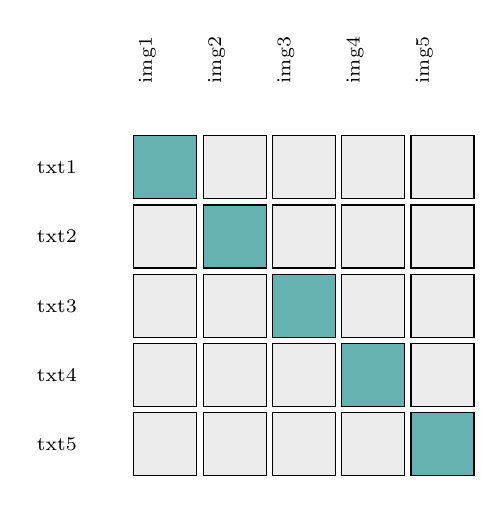
\begin{tikzpicture}[scale=0.8, every node/.style={font=\scriptsize}]
  \foreach \i in {1,...,5} {
    \node[rotate=90, anchor=south] at (\i*1.1, 0.6) {img\i};
    \node[anchor=east] at (-0.15, -\i*1.1) {txt\i};
  }
  \foreach \i in {1,...,5} {
    \foreach \j in {1,...,5} {
      \ifnum\i=\j
        \draw[fill=teal!60] (\i*1.1-0.5, -\j*1.1-0.5) rectangle ++(1,1);
      \else
        \draw[fill=gray!15] (\i*1.1-0.5, -\j*1.1-0.5) rectangle ++(1,1);
      \fi
    }
  }
\end{tikzpicture}
\end{center}

\begin{itemize}
  \item Every image is shown every caption in the batch, and gets a similarity score against each. Training pushes the \textcolor{teal}{correct pair} (the diagonal, teal) toward the highest score in its row \emph{and} its column, and every other combination (gray) toward a low score.
  \item The bigger the batch, the more ``wrong nametags'' each image is contrasted against per step, for free -- which is exactly why CLIP trains with very large batches (tens of thousands of pairs): more negatives per positive means a sharper, more informative training signal.
  \item Nothing here is unique to images and text -- the same trick trains a dual encoder for any two things you want a shared similarity space over (e.g.\ audio clips and their descriptions).
\end{itemize}
\end{vbframe}

\begin{vbframe}{Pattern 2: Fusion Architectures}
\begin{itemize}
  \item Instead of two independent towers, run modality-specific encoders and then let a shared component attend across \emph{both} -- e.g.\ \textbf{UniT} (Hu \& Singh, 2021): a BERT-style text encoder and a DETR-style vision encoder, whose outputs are concatenated into one sequence and fed to a shared decoder, together with a task-specific query.
  \item Trade-off versus dual encoders: slower (no pre-computable embeddings, the whole model runs per query), but able to model token-to-token interactions between modalities -- necessary for tasks that need fine-grained grounding, e.g.\ visual question answering (``what color is the object left of the dog?'' needs the model to actually align specific words with specific regions).
  \item General pattern: \textbf{dual-encoder/contrastive when you need fast retrieval or zero-shot matching} (CLIP-style); \textbf{fusion when the task needs the two modalities to actually interact}.
\end{itemize}
{\footnotesize Framing after the LMU Multimodal Deep Learning seminar (\href{https://slds-lmu.github.io/seminar_multimodal_dl/}{slds-lmu.github.io/seminar\_multimodal\_dl}), licensed CC BY-NC-SA 4.0.}
\end{vbframe}

\begin{vbframe}{Telling the Two Patterns Apart, By Task}
\begin{itemize}
  \item \textbf{``Find me photos similar to this one'' (reverse image search):} embed every photo in the database once, offline, with a dual encoder; at query time just embed the new photo and rank by similarity. Millions of comparisons per second, because nothing needs to be recomputed per query -- this is precisely what a dual encoder is good at, and precisely why fusion would be far too slow here (it would have to rerun the whole model for every candidate).
  \item \textbf{``What color is the object to the left of the dog?'' (visual question answering):} answering this requires the model to locate ``the dog'', reason about ``to the left of'', and check color -- all specific, fine-grained interactions between particular words and particular image regions. A dual encoder only ever produces two whole-image/whole-sentence summary vectors and compares them once at the end; by the time it does, the specific spatial relationship the question asks about has already been averaged away. Fusion, which lets word-tokens and patch-tokens attend to each other directly, is what actually has a chance at this.
  \item The pattern generalizes past vision-language: it's the same distinction as document retrieval (dual-encoder embeddings, fast, coarse) versus a re-ranker that reads the query and each candidate document together (fusion, slow, precise) -- systems in practice often use both in sequence, a dual encoder to shortlist candidates cheaply, then fusion to re-rank the shortlist accurately.
\end{itemize}
\end{vbframe}

\begin{vbframe}{Image Captioning: Encoder-Decoder, Again}
\begin{itemize}
  \item Image captioning (image in, descriptive text out) is naturally an \textbf{encoder-decoder} task -- the same pattern as T5 and Whisper, just with an image encoder instead of a text or audio one.
  \item History: CNN features $\to$ RNN decoder (pre-attention) $\to$ CNN features $+$ an attention mechanism over spatial regions (\emph{Show, Attend and Tell}, Xu et al., 2016 -- already seen as a case study in session 7's Attention section) $\to$ today, a full Transformer: self-attention encoder over image-patch features, decoder with masked self-attention over words plus cross-attention over the encoder's output.
\end{itemize}

\framebreak

\textbf{One refinement worth naming:} the \textbf{Meshed-Memory Transformer} (M$^2$, Cornia et al., 2020), a captioning-specific state-of-the-art at its time.
\begin{itemize}
  \item \textbf{Memory-augmented attention} (encoder side): append extra, purely-learnable key/value vectors to the ones computed from the image -- slots the model can use to store generic, dataset-level visual/semantic priors (``a plate usually has food on it'') that aren't specific to any one image.
  \item \textbf{Meshed cross-attention} (decoder side): instead of only cross-attending to the \emph{final} encoder layer (as T5/Whisper do), attend to \emph{every} encoder layer's output and combine them with learned, sigmoid-gated weights -- low-level and high-level visual features both stay directly reachable from the decoder.
  \item Nothing here changes the encoder-decoder \emph{pattern} from session 7 -- both are extensions of where keys/values come from, not new attention mechanics.
\end{itemize}
\end{vbframe}

\begin{vbframe}{Text-to-Image Generation: The Short Version}
\begin{itemize}
  \item Text-to-image models (text in, image out) invert the captioning direction, and the connection to this session is the same either way: the text conditions image generation via \textbf{cross-attention} -- the query-from-one-sequence / key-and-value-from-another-sequence recipe from session 7, wherever it appears in the pipeline.
  \item \textbf{Pre-Transformer}: text-conditioned GANs (StackGAN, AttnGAN) -- a GAN generator conditioned on a text embedding, with attention (AttnGAN) letting individual image regions attend to individual words.
  \item \textbf{DALL-E 1} (Ramesh et al., 2021): an autoregressive Transformer (GPT-style, session 9's family) generating discrete image tokens (from a VQ-VAE codebook) one at a time, conditioned on preceding text tokens -- text-to-image as plain next-token prediction, at the cost of being slow to sample from.
\end{itemize}
\end{vbframe}

\begin{vbframe}{Text-to-Image Generation: The Diffusion Era}
\begin{itemize}
  \item \textbf{GLIDE} and \textbf{DALL-E 2 (unCLIP)} switch to \textbf{diffusion models} (session 6): at every denoising step, the partially-generated image cross-attends to the text's token embeddings (GLIDE), or the diffusion model is conditioned on a CLIP image embedding predicted from the text embedding by a separate ``prior'' network (DALL-E 2's two-stage design) -- CLIP's dual encoders (this session, Pattern 1) repurposed as a conditioning signal rather than for classification.
  \item \textbf{Imagen} (Saharia et al., 2022) conditions diffusion directly on a large \emph{frozen} pretrained \textbf{T5} text encoder -- session 8's flagship encoder-decoder model, reused here purely for its encoder half -- and finds a bigger, better-trained language model matters more for image quality than a bigger diffusion model.
  \item \textbf{Parti} (Yu et al., 2022) goes the other direction: autoregressive like DALL-E 1, but with a much larger ViT-VQGAN image tokenizer and model scale -- the diffusion-vs-autoregressive split for image generation mirrors this whole course's encoder/decoder-family distinctions, not a settled question.
  \item Open-source note: \textbf{Stable Diffusion} popularized running the diffusion process in a compressed \emph{latent} space (a pretrained autoencoder's bottleneck) instead of raw pixels -- the main reason it's cheap enough to run on a single consumer GPU.
\end{itemize}
{\footnotesize Framing after the LMU Multimodal Deep Learning seminar, \enquote{Text-to-Image Generation}, CC BY-NC-SA 4.0.}
\end{vbframe}

%%%%%%%%%%%%%%%%%%%%%%%%%%%%%%%%%%%%%%%%%%%%%%%%%%%%%%%%%%%%%%%%%%

\section{Unified, Domain-Agnostic Architectures}
%%%%%%%%%%%%%%%%%%%%%%%%%%%%%%%%%%%%%%%%%%%%%%%%%%%%%%%%%%%%%%%%%%

\begin{vbframe}{One Model, Any Modality: Gato}
\begin{itemize}
  \item \textbf{Gato} (Reed et al., 2022): a single \textbf{decoder-only} Transformer -- the same family as GPT (session 9) -- trained on text, images, robot joint-actions, and Atari game observations, all at once.
  \item The trick is entirely in the tokenization, not the architecture: every modality is serialized into a flat token sequence (images: ViT-style patches; continuous actions: discretized into tokens; a separator token \texttt{|} marks the boundary between an observation and the action taken in response), then it's just next-token prediction, exactly like any GPT-style model.
  \item If a Transformer decoder is just ``predict the next token given the previous ones,'' and \emph{anything} can be serialized into tokens, the architecture itself was never specific to language -- language was simply the first domain where tokenization was obvious.
\end{itemize}
\end{vbframe}

\begin{vbframe}{What One Gato Training Example Actually Looks Like}
\begin{center}
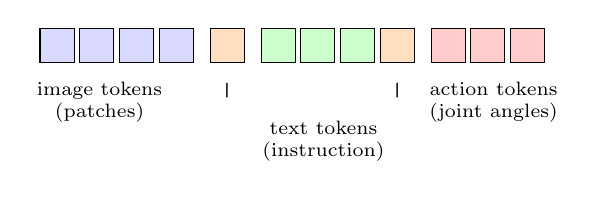
\begin{tikzpicture}[scale=0.72, every node/.style={font=\scriptsize}]
  \foreach \i in {0,...,3} { \draw[fill=blue!15] (\i*0.7,0) rectangle ++(0.6,0.6); }
  \node[align=center] at (1.05,-0.7) {image tokens\\(patches)};
  \draw[fill=orange!25] (3.0,0) rectangle ++(0.6,0.6);
  \node at (3.3,-0.5) {\texttt{|}};
  \foreach \i in {0,...,2} { \draw[fill=green!20] (3.9+\i*0.7,0) rectangle ++(0.6,0.6); }
  \node[align=center] at (5.0,-1.4) {text tokens\\(instruction)};
  \draw[fill=orange!25] (6.0,0) rectangle ++(0.6,0.6);
  \node at (6.3,-0.5) {\texttt{|}};
  \foreach \i in {0,...,2} { \draw[fill=red!20] (6.9+\i*0.7,0) rectangle ++(0.6,0.6); }
  \node[align=center] at (8.0,-0.7) {action tokens\\(joint angles)};
\end{tikzpicture}
\end{center}
\begin{itemize}
  \item One single flat sequence: a camera image (patchified exactly like ViT), then a separator {\tt |}, then a text instruction (``pick up the red block''), another separator, then a robot arm's next action (discretized into tokens, the same way a continuous pixel value or an image patch already gets discretized/embedded elsewhere in this course).
  \item The model has no idea (and no architectural mechanism to know) that some of these tokens ``are” pixels and others ``are” joint angles -- to the Transformer, it is one sequence, and the loss is the same next-token prediction loss GPT uses on pure text.
  \item This is why Gato needs no vision-specific or robotics-specific submodule: all of the domain-specific work happens once, at tokenization, before the Transformer ever sees the data.
\end{itemize}
\end{vbframe}

\begin{vbframe}{OFA: One Seq2Seq Model, Any Task}
\begin{itemize}
  \item \textbf{OFA} (``Once For All'', Wang et al., 2022) takes the text-to-text idea from session 8's T5 and pushes it across modalities: \emph{every} input and output -- text, image patches, bounding-box coordinates -- is sequentialized into one shared vocabulary and processed by a single encoder-decoder Transformer.
  \item Image patches are tokenized the same way DALL-E's discrete image tokens work (each patch maps to one of a fixed codebook of visual tokens), so images and text share one token space instead of needing separate embedding tables.
  \item This unifies \emph{understanding} tasks (captioning, VQA -- output is text) and \emph{generation} tasks (text-to-image -- output is image tokens) as literally the same kind of seq2seq problem, distinguished only by a task-instruction prefix, exactly like T5's task prefixes.
\end{itemize}
\end{vbframe}

\begin{vbframe}{The Landscape, Briefly}
\begin{itemize}
  \item \textbf{UniT} (fusion, seen above) and \textbf{OFA} (unified seq2seq, previous frame) both sequentialize modalities into a shared representation -- they differ in whether the decoder is task-specific (UniT) or the task itself is described in the input (OFA).
  \item \textbf{LIMoE} (Mustafa et al., 2022): keeps modality-specific processing not via separate encoders, but via a \textbf{mixture-of-experts} layer -- each token (regardless of modality) is routed to whichever few experts (out of many) suit it best, letting the model specialize internally without hand-splitting the architecture by modality.
  \item Common theme across all of these and Gato: the architectural primitives from session 7 (self-attention, positional encoding) stay fixed; what differs is only \emph{how a given modality gets turned into tokens} in the first place.
\end{itemize}
{\footnotesize Framing after the LMU Multimodal Deep Learning seminar, \enquote{Multi-Purpose Models}, CC BY-NC-SA 4.0.}
\end{vbframe}

%%%%%%%%%%%%%%%%%%%%%%%%%%%%%%%%%%%%%%%%%%%%%%%%%%%%%%%%%%%%%%%%%%

\section{Video: One More Dimension}
%%%%%%%%%%%%%%%%%%%%%%%%%%%%%%%%%%%%%%%%%%%%%%%%%%%%%%%%%%%%%%%%%%

\begin{vbframe}{The Problem: Video Adds a Time Axis}
\begin{itemize}
  \item A video is a sequence of frames -- the most direct extension of ViT patchifies \emph{space and time together}: a small spatial patch spanning a handful of consecutive frames (a ``tubelet'') becomes one token, instead of one flat image patch.
  \item This multiplies sequence length by the number of frames sampled, which makes the $\mathcal{O}(n^2)$ self-attention cost from session 7 far worse than for a single image -- attending every space-time patch to every other one is usually not affordable.
  \item No new architectural primitive is needed to solve this -- just session 7's efficient-attention toolbox (local/factorized patterns), applied to a harder instance of the same problem.
\end{itemize}
\end{vbframe}

\begin{vbframe}{ViViT: Four Ways to Factor Space and Time}
\citebutton{Arnab et al., 2021}{https://arxiv.org/abs/2103.15691} propose four variants, trading accuracy against cost:
\begin{itemize}
  \item \textbf{Spatio-temporal attention}: attend jointly over every space-time patch. Best accuracy, cost $\mathcal{O}(n_h^2 n_w^2 n_t^2)$ -- the expensive, unfactorized baseline.
  \item \textbf{Factorised encoder}: run an ordinary spatial ViT independently per frame, then a separate, small temporal Transformer over the resulting per-frame summary tokens. Cheaper ($\mathcal{O}(n_h^2 n_w^2 + n_t^2)$), because space and time are handled sequentially rather than jointly.
  \item \textbf{Factorised self-attention} and \textbf{factorised dot-product attention}: stay within one block, but split attention into a spatial pass and a temporal pass (either sequentially, or across different attention heads) rather than factorizing into two separate sub-networks.
\end{itemize}

\framebreak

\textbf{An intuition for factorizing:} think about how \emph{you} understand a movie scene.
\begin{center}
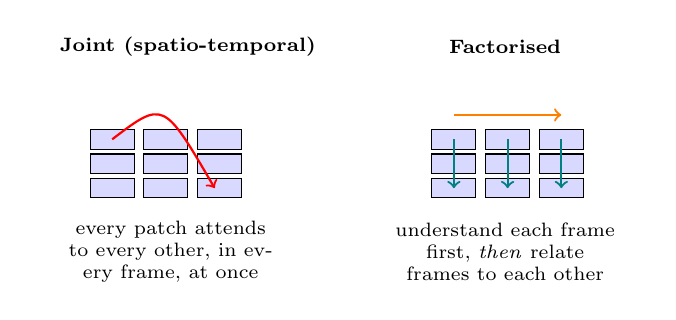
\begin{tikzpicture}[scale=0.62, every node/.style={font=\scriptsize}]
  \node at (2,3.4) {\textbf{Joint (spatio-temporal)}};
  \foreach \f in {0,1,2} {
    \foreach \p in {0,1,2} {
      \draw[fill=blue!15] (\f*1.1, \p*0.5+0.3) rectangle ++(0.9,0.4);
    }
  }
  \draw[->, red, thick] (0.45,1.5) .. controls (1.5,2.3) .. (2.55,0.5);
  \node[align=center, text width=3.4cm] at (1.65,-0.8) {every patch attends to every other, in every frame, at once};

  \node at (8.5,3.4) {\textbf{Factorised}};
  \foreach \f in {0,1,2} {
    \foreach \p in {0,1,2} {
      \draw[fill=blue!15] (7+\f*1.1, \p*0.5+0.3) rectangle ++(0.9,0.4);
    }
    \draw[->, teal, thick] (7+\f*1.1+0.45,1.5) -- (7+\f*1.1+0.45,0.5);
  }
  \draw[->, orange, thick] (7.45,2.0) -- (9.65,2.0);
  \node[align=center, text width=3.4cm] at (8.5,-0.8) {understand each frame first, \emph{then} relate frames to each other};
\end{tikzpicture}
\end{center}
\begin{itemize}
  \item \textbf{Joint attention} is like staring at all frames superimposed on top of each other simultaneously, trying to spot every relationship between every pixel in every frame at once -- accurate in principle, but an enormous amount to process together.
  \item \textbf{Factorised attention} is what you actually do: first understand what's happening \emph{within} each frame (spatial), then track how that understanding \emph{changes across} frames (temporal) -- two much smaller problems solved one after the other, instead of one huge problem solved all at once.
\end{itemize}
\end{vbframe}

\begin{vbframe}{Getting Tokens from Video}
\begin{itemize}
  \item \textbf{Uniform frame sampling}: take every $k$-th frame, patchify each independently, exactly like a batch of images -- simple, but temporal information only enters through the attention pattern, never through tokenization itself.
  \item \textbf{Tubelet embedding}: each token's linear projection spans a small 3D space-time volume directly, so adjacent-frame information is fused \emph{before} the first attention layer even runs -- a strictly richer starting representation, at the cost of a slightly more involved patch-extraction step.
\end{itemize}
\end{vbframe}

\begin{vbframe}{TimeSformer: Divided Space-Time Attention}
\begin{itemize}
  \item Concurrent work \citebutton{Bertasius et al., 2021}{https://arxiv.org/abs/2102.05095} tried five different attention schemes for video and found \textbf{divided space-time attention} the best trade-off: within each block, first attend over space (same frame, all positions), then over time (same position, all frames) -- sequentially divided, not a single joint operation.
  \item Same underlying idea as ViViT's factorised variants, arrived at independently: joint spatio-temporal attention is rarely worth its cost once you can factor the two axes apart.
\end{itemize}
{\footnotesize Framing after Hugging Face's Community Computer Vision Course, Unit 7 \enquote{Video Processing} (MIT licensed).}
\end{vbframe}

%%%%%%%%%%%%%%%%%%%%%%%%%%%%%%%%%%%%%%%%%%%%%%%%%%%%%%%%%%%%%%%%%%

\section{Closing Synthesis: Four Sessions, One Architecture}
%%%%%%%%%%%%%%%%%%%%%%%%%%%%%%%%%%%%%%%%%%%%%%%%%%%%%%%%%%%%%%%%%%

\begin{vbframe}{The Complete Map}
\begin{center}
\footnotesize
\begin{tabular}{@{}p{1.7cm}p{3.0cm}p{2.6cm}p{3.4cm}@{}}
\toprule
 & \textbf{Encoder-only} & \textbf{Decoder-only} & \textbf{Encoder-decoder} \\
\midrule
NLP & BERT, RoBERTa, ALBERT, DistilBERT, ELECTRA & GPT (session 9) & original Transformer, T5 \\[4pt]
Vision & Vision Transformer & autoregressive image generation & DETR (parallel, non-autoregressive decoding) \\[4pt]
Audio & wav2vec 2.0-style encoders & -- & Whisper \\[4pt]
Cross-modal / unified & CLIP (dual-encoder) & Gato (any modality as tokens) & captioning, text-to-image cross-attention, UniT/OFA (fusion) \\
\bottomrule
\end{tabular}
\end{center}
\begin{itemize}
  \item Four sessions, one small set of ideas: self-attention as content-based routing, positional encoding to recover order, and three attention patterns (bidirectional, causal, cross) that combine into three architecture families -- everything else in this table is a choice of \emph{what gets tokenized} and \emph{which objective trains it}.
  \item Session 11 changes topic entirely: reinforcement learning.
\end{itemize}
\end{vbframe}

%%%%%%%%%%%%%%%%%%%%%%%%%%%%%%%%%%%%%%%%%%%%%%%%%%%%%%%%%%%%%%%%%%
%%%%%%%%%%%%%%%%%%          REFERENCES          %%%%%%%%%%%%%%%%%%
%%%%%%%%%%%%%%%%%%%%%%%%%%%%%%%%%%%%%%%%%%%%%%%%%%%%%%%%%%%%%%%%%%
\begin{vbframe}
\frametitle{References}
\footnotesize{
\begin{thebibliography}{99}
\bibitem[(Dosovitskiy et al., 2020)]{o1} Dosovitskiy, A. et al.\ (2020). \textit{An Image is Worth 16x16 Words: Transformers for Image Recognition at Scale}. \url{https://arxiv.org/abs/2010.11929}
\bibitem[(Carion et al., 2020)]{o2} Carion, N. et al.\ (2020). \textit{End-to-End Object Detection with Transformers (DETR)}. \url{https://arxiv.org/abs/2005.12872}
\bibitem[(Zhu et al., 2020)]{o3} Zhu, X. et al.\ (2020). \textit{Deformable DETR}. \url{https://arxiv.org/abs/2010.04159}
\bibitem[(Meng et al., 2021)]{o4} Meng, D. et al.\ (2021). \textit{Conditional DETR for Fast Training Convergence}. \url{https://arxiv.org/abs/2108.06152}
\bibitem[(Radford et al., 2021)]{o5} Radford, A. et al.\ (2021). \textit{Learning Transferable Visual Models From Natural Language Supervision (CLIP)}. \url{https://arxiv.org/abs/2103.00020}
\bibitem[(Hu \& Singh, 2021)]{o6} Hu, R., \& Singh, A. (2021). \textit{UniT: Multimodal Multitask Learning with a Unified Transformer}. \url{https://arxiv.org/abs/2102.10772}
\bibitem[(Xu et al., 2016)]{o7} Xu, K. et al.\ (2016). \textit{Show, Attend and Tell}. \url{https://arxiv.org/abs/1502.03044}
\bibitem[(Saharia et al., 2022)]{o8} Saharia, C. et al.\ (2022). \textit{Photorealistic Text-to-Image Diffusion Models with Deep Language Understanding (Imagen)}. \url{https://arxiv.org/abs/2205.11487}
\bibitem[(Reed et al., 2022)]{o9} Reed, S. et al.\ (2022). \textit{A Generalist Agent (Gato)}. \url{https://arxiv.org/abs/2205.06175}
\bibitem[(Wang et al., 2022)]{o10} Wang, P. et al.\ (2022). \textit{OFA: Unifying Architectures, Tasks, and Modalities Through a Simple Sequence-to-Sequence Learning Framework}. \url{https://arxiv.org/abs/2202.03052}
\bibitem[(Mustafa et al., 2022)]{o11} Mustafa, B. et al.\ (2022). \textit{Multimodal Contrastive Learning with LIMoE}. \url{https://arxiv.org/abs/2206.02770}
\bibitem[(Redmon et al., 2015)]{o12} Redmon, J. et al.\ (2015). \textit{You Only Look Once (YOLO)}. \url{https://arxiv.org/abs/1506.02640}
\bibitem[(Liu et al., 2021)]{o13} Liu, Z. et al.\ (2021). \textit{Swin Transformer: Hierarchical Vision Transformer using Shifted Windows}. \url{https://arxiv.org/abs/2103.14030}
\bibitem[(Touvron et al., 2021)]{o14} Touvron, H. et al.\ (2021). \textit{Training Data-Efficient Image Transformers \& Distillation Through Attention (DeiT)}. \url{https://arxiv.org/abs/2012.12877}
\bibitem[(Cheng et al., 2021)]{o15} Cheng, B., Schwing, A., \& Kirillov, A. (2021). \textit{Per-Pixel Classification is Not All You Need for Semantic Segmentation (MaskFormer)}. \url{https://arxiv.org/abs/2107.06278}
\bibitem[(Arnab et al., 2021)]{o16} Arnab, A. et al.\ (2021). \textit{ViViT: A Video Vision Transformer}. \url{https://arxiv.org/abs/2103.15691}
\bibitem[(Bertasius et al., 2021)]{o17} Bertasius, G., Wang, H., \& Torresani, L. (2021). \textit{Is Space-Time Attention All You Need for Video Understanding? (TimeSformer)}. \url{https://arxiv.org/abs/2102.05095}
\bibitem[(Cornia et al., 2020)]{o18} Cornia, M. et al.\ (2020). \textit{Meshed-Memory Transformer for Image Captioning}. \url{https://arxiv.org/abs/1912.08226}
\bibitem[(Ramesh et al., 2021)]{o19} Ramesh, A. et al.\ (2021). \textit{Zero-Shot Text-to-Image Generation (DALL-E)}. \url{https://arxiv.org/abs/2102.12092}
\bibitem[(Nichol et al., 2021)]{o20} Nichol, A. et al.\ (2021). \textit{GLIDE: Towards Photorealistic Image Generation and Editing with Text-Guided Diffusion Models}. \url{https://arxiv.org/abs/2112.10741}
\bibitem[(Ramesh et al., 2022)]{o21} Ramesh, A. et al.\ (2022). \textit{Hierarchical Text-Conditional Image Generation with CLIP Latents (DALL-E 2 / unCLIP)}. \url{https://arxiv.org/abs/2204.06125}
\bibitem[(Yu et al., 2022)]{o22} Yu, J. et al.\ (2022). \textit{Scaling Autoregressive Models for Content-Rich Text-to-Image Generation (Parti)}. \url{https://arxiv.org/abs/2206.10789}
\bibitem[(Rombach et al., 2022)]{o23} Rombach, R. et al.\ (2022). \textit{High-Resolution Image Synthesis with Latent Diffusion Models (Stable Diffusion)}. \url{https://arxiv.org/abs/2112.10752}
\end{thebibliography}
}
\end{vbframe}

%%%%%%%%%%%%%%%%%%%%%%%%%%%%%%%%%%%%%%%%%%%%%%%%%%%%%%%%%%%%%%%%%%
\section{License \& Attribution}
%%%%%%%%%%%%%%%%%%%%%%%%%%%%%%%%%%%%%%%%%%%%%%%%%%%%%%%%%%%%%%%%%%

\begin{vbframe}{License \& Attribution}
\begin{itemize}
\item Unlike sessions 7-8, no content in this session is adapted from i2dl or DL4NLP (neither course covers non-NLP Transformer applications). All frames are freshly written for this course, since none of the source material below is in Beamer slide form.
\item The \enquote{Vision Transformers, In Depth}, \enquote{Efficient Vision Transformers} (Swin, DeiT), \enquote{DETR}, and \enquote{Segmentation Transformers} sections follow the explanations (and, for the DETR code frame, the code) of the \textbf{Hugging Face Community Computer Vision Course} (\url{https://github.com/huggingface/computer-vision-course}) --- licensed \textbf{MIT}, verified directly from the repository's license file. DeiT's specific mechanism (the distillation token) is stated from general knowledge of the original paper, not from the course's own (more general) knowledge-distillation chapter, which does not describe DeiT specifically.
\item The \enquote{Video} section (ViViT's four variants, tubelet embedding, TimeSformer) also follows the same Hugging Face course, Unit 7 \enquote{Video Processing} --- same MIT license.
\item The \enquote{Combining Modalities} and \enquote{Unified, Domain-Agnostic Architectures} sections (incl.\ OFA) follow the \textbf{LMU Multimodal Deep Learning seminar} (\url{https://slds-lmu.github.io/seminar_multimodal_dl/}) --- licensed \textbf{CC BY-NC-SA 4.0} (confirmed in the book's own front matter), the same license class already carried by session 7's Fleuret-derived material: non-commercial academic teaching is covered, but reuse must be attributed and shared alike.
\item All diagrams (patch-embedding illustration, DETR architecture, dual-encoder diagram) are original TikZ, not reproductions of any source's figures --- both courses' own images were left out entirely rather than downloaded, since their individual provenance (some may originate from the original papers rather than the course authors) wasn't independently verified.
\item Stanford's CS25 (\enquote{Transformers United}) was checked for this session's scope (topic list only) and confirmed to carry \emph{no} license or reuse statement of any kind -- no content, code, or figures from it are used anywhere in this deck.
\item The closing synthesis table is original content, not adapted from any single source.
\item All worked examples and intuitive analogies added in this session's third pass (the patch-count arithmetic, the shifted-photo inductive-bias example, Swin's paragraph-shifting analogy, DETR's numeric matching example, CLIP's ``matching game'' framing and similarity-matrix diagram, the dual-encoder-vs-fusion task comparison, Gato's token-sequence diagram, and ViViT's movie-watching analogy) are freshly authored for this course, not sourced from HF or LMU -- neither course phrases these subtopics this way. Where an added frame restates a fact already cited elsewhere in this deck (e.g.\ the $224\times224$/$16\times16$ patch arithmetic follows directly from Dosovitskiy et al.'s own patch-size choice), the original citation from the earlier frame still applies; it is not repeated as a separate claim.
\end{itemize}
\end{vbframe}

\endlecture
\end{document}
